% Model 3: concise logic chain, 3 core equations, visual Discreteness & Matrix chart,
% and stress-test results aligned with Task 3 of CQU Problem B (no M1 sensitivity overlap).
\clearpage
\section{Model 3: Post-Construction Resilience under Compound Disasters}\label{sec:model3}
Task~3 asks whether the belt planned in Model~2 can withstand disasters and recover. Starting from Model~2's year~15 ($t=0$), we follow the belt for 50 more years through four links:

\begin{center}
\begin{tikzpicture}[font=\normalsize,
  chainbox/.style={draw, rounded corners=2pt, line width=0.8pt, minimum width=1.95cm, minimum height=0.88cm, align=center},
  haz/.style={chainbox, draw=pSand, fill=pSand!10, text=pSand},
  wat/.style={chainbox, draw=pWater, fill=pWater!8, text=pWater},
  veg/.style={chainbox, draw=pVeg, fill=pVeg!8, text=pVeg},
  cen/.style={chainbox, draw=pPlum, fill=pPlum!8, text=pPlum},
  lk/.style={-{Stealth[length=6pt]}, line width=1pt},
  num/.style={circle, fill=white, draw, inner sep=0.5pt, font=\scriptsize\bfseries, minimum size=12pt}]
\node[haz] (a) {$D_t^{\mathrm{dr}},\ R_t$};
\node[wat, right=1.30cm of a] (b) {$I_{j,t,m}\xrightarrow{\Phi}\widetilde V$};
\node[veg, right=1.30cm of b] (c) {$V_{j,t+1},\ M_{j,t+1}$};
\node[cen, right=1.30cm of c] (d) {$\tau_{\mathrm{proj}}\ \text{vs.}\ H_{\mathrm{eco}}$};
\draw[lk, pSand]  (a) -- node[num, draw=pSand, text=pSand] {a} (b);
\draw[lk, pWater] (b) -- node[num, draw=pWater, text=pWater] {b} (c);
\draw[lk, pPlum]  (c) -- node[num, draw=pPlum, text=pPlum] {c} (d);
\draw[lk, pVeg]   (c.south) -- ++(0,-0.45) -| (b.south);
\node[num, draw=pVeg, text=pVeg] at ($(b.south)!0.5!(c.south)+(0,-0.45)$) {d};
\end{tikzpicture}
\end{center}

\noindent \textcircled{\scriptsize a} Droughts and storms arrive at random; \textcircled{\scriptsize b} rationed canal water drives Model~1's water--cover map $\Phi$; \textcircled{\scriptsize c} each year we check whether half the belt is below the warning level; \textcircled{\scriptsize d} the stands keep growing afterwards, so they can \textbf{recover} (Figure~\ref{fig:m3-struct}).

\begin{figure}[!htb]
  \centering
  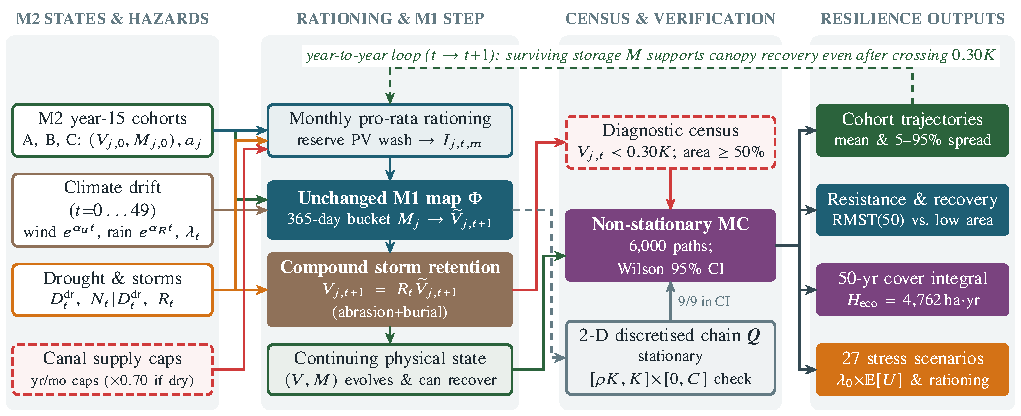
\includegraphics[width=\linewidth]{m3_structure.pdf}
  \caption{Structure of Model~3. Inherited Model~2 cohorts evolve under compound droughts, storm shocks, and monthly rationing, cross-checked against a stationary 2-D discretised Markov chain.}
  \label{fig:m3-struct}
\end{figure}

\subsection{Model construction}
\paragraph{Inherited stands and compound hazards.} Model~3 does not reset the belt to full cover. It starts from Model~2's three year-15 cohorts: \textbf{A} ($100$\,ha, $V_0=17.1\%$, $300$\,mm/yr), \textbf{B} ($50$\,ha core strip, $V_0=23.4\%$, $600$\,mm/yr) and \textbf{C} ($150$\,ha, $V_0=16.9\%$, $300$\,mm/yr), each with its own stored soil water. The four disasters of Task~3 enter through two channels so that one storm is not counted three times \cite{EN14,EN15}. \emph{Drought} is a shared yearly switch $D_t^{\mathrm{dr}}$ that cuts rain ($\times0.40$), raises demand ($\times1.15$), shrinks canal caps ($\times0.70$) and makes storms $1.5$ times more frequent; \emph{sandstorm, abrasion and burial} remove a random share of cover:
\begin{equation}\label{eq:m3-hazard}
N_t\mid D_t^{\mathrm{dr}}\sim\mathrm{Poisson}\big(\lambda_0 e^{\alpha_\lambda t}\gamma^{D_t^{\mathrm{dr}}}\big),\qquad
R_t=\prod_{q=1}^{N_t}(1-U_{t,q}),\quad U_{t,q}\sim\mathrm{U}(0.10,0.50).
\end{equation}
Climate drift slowly raises wind ($e^{\alpha_u t}$, acting through Model~1's $\mathrm{ET}_0$) and lowers rain ($e^{\alpha_R t}$).

\paragraph{One year of the belt.} Canal water is rationed month by month (PV washing first, the rest shared in proportion to requests), the unchanged Model~1 map $\Phi$ grows each cohort, and the storm retention is applied at year end:
\begin{equation}\label{eq:m3-step}
(\widetilde V_{j,t+1},\,M_{j,t+1})=\Phi\big(V_{j,t},M_{j,t};I_{j,t,m}\big),\qquad V_{j,t+1}=R_t\,\widetilde V_{j,t+1}.
\end{equation}
The belt is flagged when at least half of its area is \emph{simultaneously} below $0.30K$ ($11.4\%$ cover proxy). We report \textbf{resistance} as the mean time to this first flag within 50 years, $\mathrm{RMST}(50)=\mathbb E[\min(\tau_{\mathrm{proj}},50)]$, and \textbf{recovery} as the gap between area that has ever crossed $0.30K$ and area still below it. The flag is only a memory: the physical $(V,M)$ keeps evolving and can climb back.

\subsection{Solution approach}
We simulate $6{,}000$ Monte Carlo paths for 50 years ($3{,}000$ per sensitivity case; Table~\ref{tab:m3-par}). As an independent check we also write the belt's yearly change as a Markov chain. Figure~\ref{fig:m3-matrix} explains what its matrix means physically:
\begin{enumerate}\setlength{\itemsep}{1pt}\setlength{\parsep}{0pt}
  \item \textbf{A state is a stand's condition.} Each cell pairs a cover level $V$ with a soil-water level $M$. Both are needed: two stands with the same cover but different stored water fare differently next year. All cells below $0.30K$ merge into one ``below warning'' state.
  \item \textbf{A row lists next year's possibilities.} Row $i$ of $\bm P$ holds the chance that a stand now in cell $i$ ends next year in each cell $j$: a good year moves it towards denser cover, a drought towards drier and sparser cover, and a severe storm can drop it below the warning level.
  \item \textbf{The last column and row record the warning.} The last column is this year's chance of falling below $0.30K$; the last row keeps that flag once raised, while physical recovery is followed separately in the Monte Carlo runs. Because a stand only moves to nearby cells in one year, most entries are zero, and multiplying by $\bm P$ year after year gives the chance of being flagged within any horizon.
\end{enumerate}

\begin{figure}[!htb]
  \centering
  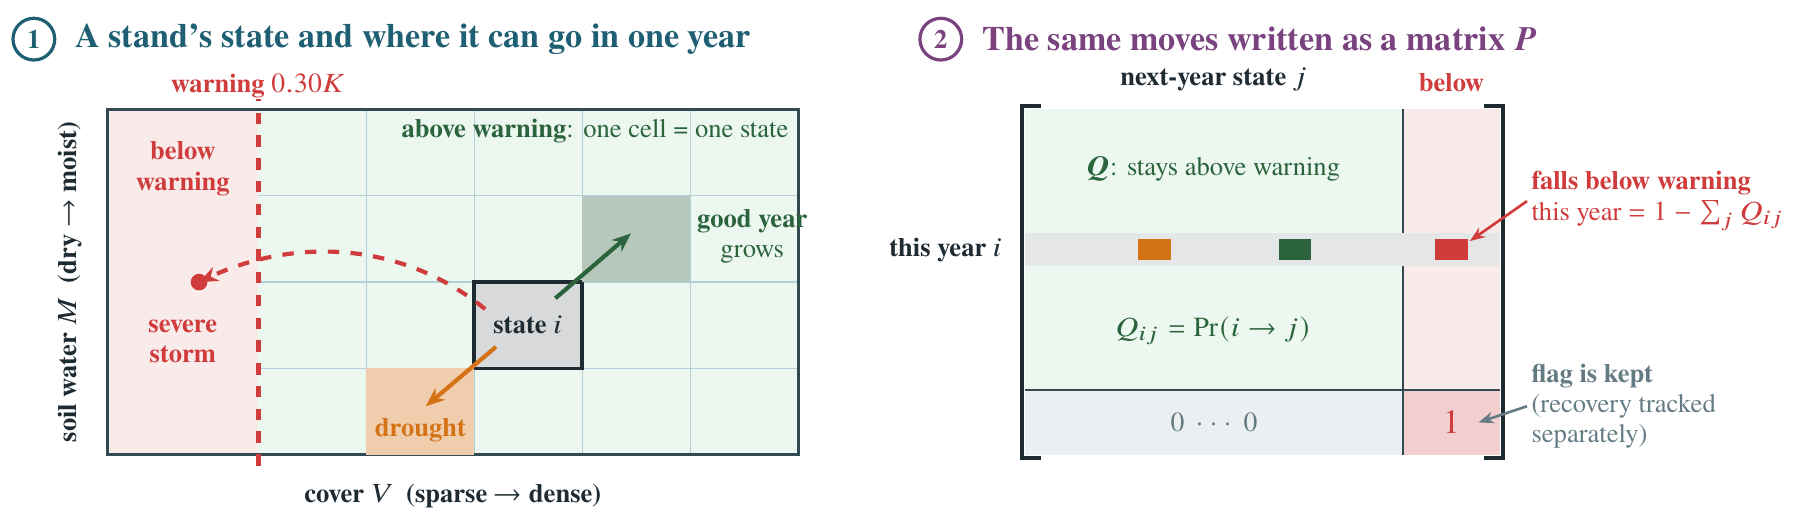
\includegraphics[width=\linewidth]{m3_matrix_discrete.png}
  \caption{Physical meaning of the transition matrix: (1) a stand's state (cover, soil water) and its typical one-year moves; (2) the same moves as one row of $\bm P$.}
  \label{fig:m3-matrix}
\end{figure}

\begin{table}[!htb]
\centering\small
\renewcommand{\arraystretch}{1.05}
\begin{tabularx}{\linewidth}{@{}l X r l@{}}
\toprule
Symbol & Meaning (stress-test scenario, not calibrated) & Base value & Tested \\
\midrule
$\lambda_0;\ U$ & storm rate; cover loss per storm & $0.25$/yr; $\mathrm{U}(0.10,0.50)$ & $3\times3$ grid \\
$p_D;\ \gamma$ & drought probability; storm multiplier in drought & $0.12{+}0.002t;\ 1.5$ & no drought; $\gamma=1$ \\
$\alpha_u,\alpha_R,\alpha_\lambda$ & yearly trends in wind, rain, storm rate & $+0.5\%,-0.5\%,+1\%$ & stationary \\
$\rho,\beta;\ H$ & flag threshold, area share; horizon & $0.30K,\ 50\%;\ 50$\,yr & $0.20K$, $0.40K$ \\
\bottomrule
\end{tabularx}
\caption{Model~3 scenario parameters.}
\label{tab:m3-par}
\end{table}

\subsection{Results}
\paragraph{The belt is hit often but recovers.} Under the baseline stress test, the belt is flagged within 10 years with probability $77.5\%$, and $\mathrm{RMST}(50)=7.1$\,yr. The $600$\,mm/yr core strip B resists more than twice as long ($16.1$\,yr) as cohorts A and C ($7.1$--$7.2$\,yr; Figure~\ref{fig:m3-res}a). A flag, however, is not a collapse: by year~50 almost all $300$\,ha has crossed $0.30K$ at some point, yet only $200$\,ha is below it, so about \textbf{$99$\,ha has recovered} on stored water and continued irrigation (Figure~\ref{fig:m3-res}b). The belt still delivers $4{,}762\text{ effective ha}\cdot\text{yr}$, $65.5\%$ of the disaster-free path (Figure~\ref{fig:m3-res}c). In drought years the canal caps bind from April to September and cut May delivery by $26\%$ (Figure~\ref{fig:m3-res}d).

\begin{figure}[!htb]
  \centering
  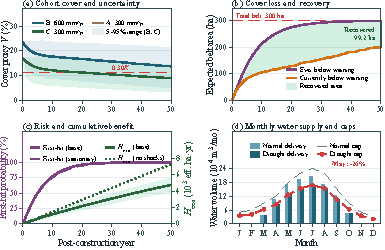
\includegraphics[width=0.96\linewidth]{m3_resilience.pdf}
  \caption{50-year stress test from Model~2's year 15 ($6{,}000$ paths, threshold $0.30K$): (a) cohort cover and 5--95\% path range, (b) ever-crossed vs.\ currently low area, (c) flag probability and cumulative cover, (d) monthly canal supply in normal and drought years.}
  \label{fig:m3-res}
\end{figure}

\paragraph{What drives the risk.} Water and wind responses were already tested in Model~1 and are not repeated. Two post-construction findings remain (Figure~\ref{fig:m3-sens}), and the numerical check confirms them:
\begin{enumerate}\setlength{\itemsep}{1pt}\setlength{\parsep}{0pt}
  \item \textbf{Storm frequency and severity dominate.} $\mathrm{RMST}(50)$ ranges from $41.8$\,yr (rare, mild storms) to $2.8$\,yr (frequent, severe storms); the baseline sits in the high-risk corner (a).
  \item \textbf{More water helps little once canals are full.} Asking for $20\%$ more water raises $\mathrm{RMST}$ only from $7.1$ to $8.1$\,yr because summer caps clip the extra request; removing droughts or the drought--storm link gains less than a year (b).
  \item \textbf{The numbers are numerically reliable.} The Markov chain lies inside the Monte Carlo $95\%$ interval at all 9 check points; refining the grid or the storm nodes changes probabilities by at most $0.04$ and $0.20$ percentage points.
\end{enumerate}

\begin{figure}[!htb]
  \centering
  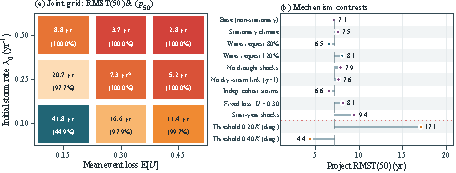
\includegraphics[width=\linewidth]{m3_sensitivity_val.pdf}
  \caption{(a) $\mathrm{RMST}(50)$ and 50-year flag probability over storm rate and loss ($^*$ uses loss range $[0.15,0.45]$); (b) project $\mathrm{RMST}(50)$ under mechanism contrasts.}
  \label{fig:m3-sens}
\end{figure}

\paragraph{Summary.} The planned belt is frequently pushed below the warning level by compound disasters, but most damage is temporary while water keeps flowing. Higher water on core strips and secure dry-summer canal supply matter more than extra annual quota.
